\ssr{ВВЕДЕНИЕ}

\textbf{Параллелизм} описывает последовательности, которые происходят одновременно \cite{posix-threads}. Таким образом параллельные вычисления таковы, что они выполняются одновременно. Распараллеливание вычислений может привести к росту временной эффективности программы при использовании на многопроцессорных и однопроцессорных, если программа часто блокируется ожиданиями ввода/вывода, системах \cite{tanenbaum}.

Некоторые программы можно разделить на части, при этом каждая такая часть выполняет определённую работу над данными и передаёт их следующей части. Таким образом образуется конвейер по обработке данных, при этом части этого конвейера могут работать параллельно друг другу.


Целью данной работы является разработка ПО, выполняющего скачивание страниц и парсинг рецептов с сайта menunedeli.ru с помощью параллельных вычислений по конвейерному принципу.

Задачами работы являются:

\begin{itemize}
	\item рассмотрение структуры сайта;
	\item разработка ПО, выполняющего парсинг рецептов в конвейере;
	\item исследование характеристик разработанного ПО на данных о интервалах времени стадий обработки рецепта.
\end{itemize}
\vspace{20mm}
{\let\clearpage\relax \chapter{Входные и выходные данные}}

Входными данными для программы являются ссылки на страницы сайта menunedeli.ru. с рецептами. Каждая ссылка содержит один рецепт в веб-ресурсе. Выходными данными являются файлы json -- загруженные рецепты по ссылкам из входных данных, при этом в каждом json файле хранится:

\begin{itemize}
	\item название рецепта;
	\item ссылка на изображение блюда;
	\item список ингредиентов;
	\item шаги рецепта.
\end{itemize}

\vspace{20mm}
{\let\clearpage\relax \chapter{Преобразование входных данных в выходные}}

Для получения ссылок с рецептами с сайта в виде файла разработан скрипт parse.py на языке python3 \cite{python3}:

\begin{lstlisting}[label=parse,caption={parse.py -- скрипт для получения ссылок с рецептами}]
	import requests as re
	import bs4
	import argparse
	import sys
	
	parser = argparse.ArgumentParser(
	prog="parse",
	description="Скачивает ссылки на статьи с сайта menunedeli.ru"
	)
	parser.add_argument("-c", "--count", type=int, default=1000, help="Количество ссылок для скачивания")
	parser.add_argument("-s", "--save", type=str, default="links.txt", help="Файл, куда сохранять ссылки")
	
	args = parser.parse_args()
	
	saveTo = args.save
	UpToLinks = args.count
	catalogFormat = "https://menunedeli.ru/novye-stati/page/{}"
	with open(saveTo, "w") as f:
		links = 0
		page = 1
		while True:
			catalogPage = re.get(catalogFormat.format(page))
	
			bs = bs4.BeautifulSoup(catalogPage.content, "lxml")
	
			for a in bs.find_all('article'):
				for link in a.find_all('meta', attrs={'itemprop':'url'}):
					if link['content'].startswith("https://menunedeli.ru/recipe"):
						print(link['content'], file=f)
						links += 1
						if links >= UpToLinks:
							exit(0)
			page += 1
\end{lstlisting}

Полученный в результате работы программы \ref{parse} файл выступает входными данными для разработанного ПО.

Основная часть программы написана на языке GO \cite{go} использую паттерн проектирования конвейер (pipeline) \cite{go-design}. Конвейер состоит из 3-х частей:

\begin{enumerate}
	\item скачивание страницы;
	\item вычленение из страницы частей рецепта (парсинг);
	\item сохранение рецепта в базе данных.
\end{enumerate}

Каждая из частей запускается в отдельной горутине (goroutine) \cite{go-mem}, которые передают данные через каналы (channel) \cite{go-mem}

Элементом данных выступает структура, которая хранит в себе информацию о рецепте, информацию о моментах времени начала и конца обработки отдельной частью программы и метаинформацию для обработчиков конвейера. Структура представлена в листинге \ref{unit}.

\begin{lstlisting}[label=unit,caption={Данные, передающиеся между частями конвейера},language=go]
	// Передаётся между частями конвейера
	type PipelineUnit struct {
		recipedb.Recipe
		PipelineTimes
		PageReader io.ReadCloser
		Err        error
	}
	
	type Ingredient struct {
		Name   string
		Amount string
		Unit   string
	}
	
	type Recipe struct {
		ID          int64
		IssueID     int64
		Url         string
		Title       string
		ImageURL    string
		Ingredients []Ingredient
		Steps       []string
	}
	
	type PipelineTimes struct {
		LoadingStart time.Time
		LoadingEnd   time.Time
		ParsingStart time.Time
		ParsingEnd   time.Time
		StorageStart time.Time
		StorageEnd   time.Time
	}
\end{lstlisting}

Полученные в результате работы программы рецепты сохраняются в базе данных PostgreSQL \cite{pgs}, а из неё отдельным скриптом сохраняются в виде json-файла.

\vspace{20mm}
{\let\clearpage\relax \chapter{Примеры работы программы}}

Один из примеров обработки веб-страниц \cite{receipt} представлен на рисунке \ref{before} и листинге \ref{after}.

\begin{figure}[h]
	\centering
	
\includegraphics[width=0.9\textwidth]{before}
	\caption{Веб-страница по ссылке \cite{receipt}}
	\label{before}
\end{figure}

\begin{lstlisting}[label=after,caption={json рецепта после обработки}]
	{
		"ID": 528,
		"ImageURL": "https://menunedeli.ru/wp-content/uploads/2024/03/Bliny-s-tvorogom-recept-nachinki-500х350.jpg-500x333.jpg?v=1710428422",
		"Ingredients": [
		{
			"Amount": "500",
			"Name": "Творог",
			"Unit": "г"
		},
		{
			"Amount": "80",
			"Name": "Сахар",
			"Unit": "г"
		},
		{
			"Amount": "1",
			"Name": "Яйцо куриное",
			"Unit": "шт."
		},
		{
			"Amount": "2",
			"Name": "Сметана",
			"Unit": "ст.л."
		},
		{
			"Amount": "0.5",
			"Name": "Цедра апельсина",
			"Unit": "ч.л."
		},
		{
			"Amount": "",
			"Name": "Ваниль",
			"Unit": "по вкусу"
		}
		],
		"IssueID": 9161,
		"Steps": [
		"...",
		"...",
		...
		],
		"Title": "Блины с творогом: рецепт начинки",
		"Url": "https://menunedeli.ru/recipe/bliny-s-tvorogom-recept-nachinki/"
	}
\end{lstlisting}
\vspace{20mm}
{\let\clearpage\relax \chapter{Тестирование}}

Тестирование программы проводилось загрузкой в качестве входных данных 1000 ссылок на различные рецепты веб-ресурса menunedeli.ru. При этом отслеживалось количество удачных скачиваний и обработок страницы, а также выборочная ручная проверка 10 случайных выходных файлов. 

Тестирование было успешно пройдено.

\vspace{20mm}
{\let\clearpage\relax \chapter{Описание исследования}}

Технические характеристики устройства,на котором выполнялась программа:

\begin{itemize}
	\item процессор: AMD Ryzen 7 5800H (16) @ 4.46 ГГц;
	\item оперативная память: 16 ГБ;
	\item операционная система: Arch Linux x86\_64.
\end{itemize}

На вход программе был подан файл с 1000 ссылок на рецепты сайта menunedeli.ru, каждая из которых была успешно обработана.

Во время выполнения, в программе фиксируются моменты времени начала и конца обработки рецепта очередным этапом конвейера. Перед окончанием программы эти данные сохраняются в отдельный файл. Часть этого файла представлена в листинге \ref{log}.

\begin{lstlisting}[label=log, caption={Часть лога, сформированного конвейром}]
	3	loading	0.184901	0.209007
	2	storage	0.205416	0.227645
	4	loading	0.209011	0.246545
	3	parsing	0.209074	0.228591
	3	storage	0.228596	0.237616
	5	loading	0.246548	0.281826
	4	parsing	0.246586	0.263061
	4	storage	0.263066	0.282869
\end{lstlisting}
Где 1-й столбец -- идентификатор заявки, 2-ой -- тип обработчика, 3-й -- начало обработки, 4-й -- конец обработки.

Из лога \ref{log} можно увидеть, что в случае конвейерной обработки может быть простой отдельных её частей, например после окончания обработки заявки 3, storage простаивает до окончания обработки 4-ой заявки обработчиком parsing. Соответственно storage простаивает между 0.237616 и 0.263066.

Простои обработчиков и части лога \ref{log} можно увидеть на рисунке \ref{timediag}

\begin{figure}[h]
	\centering
	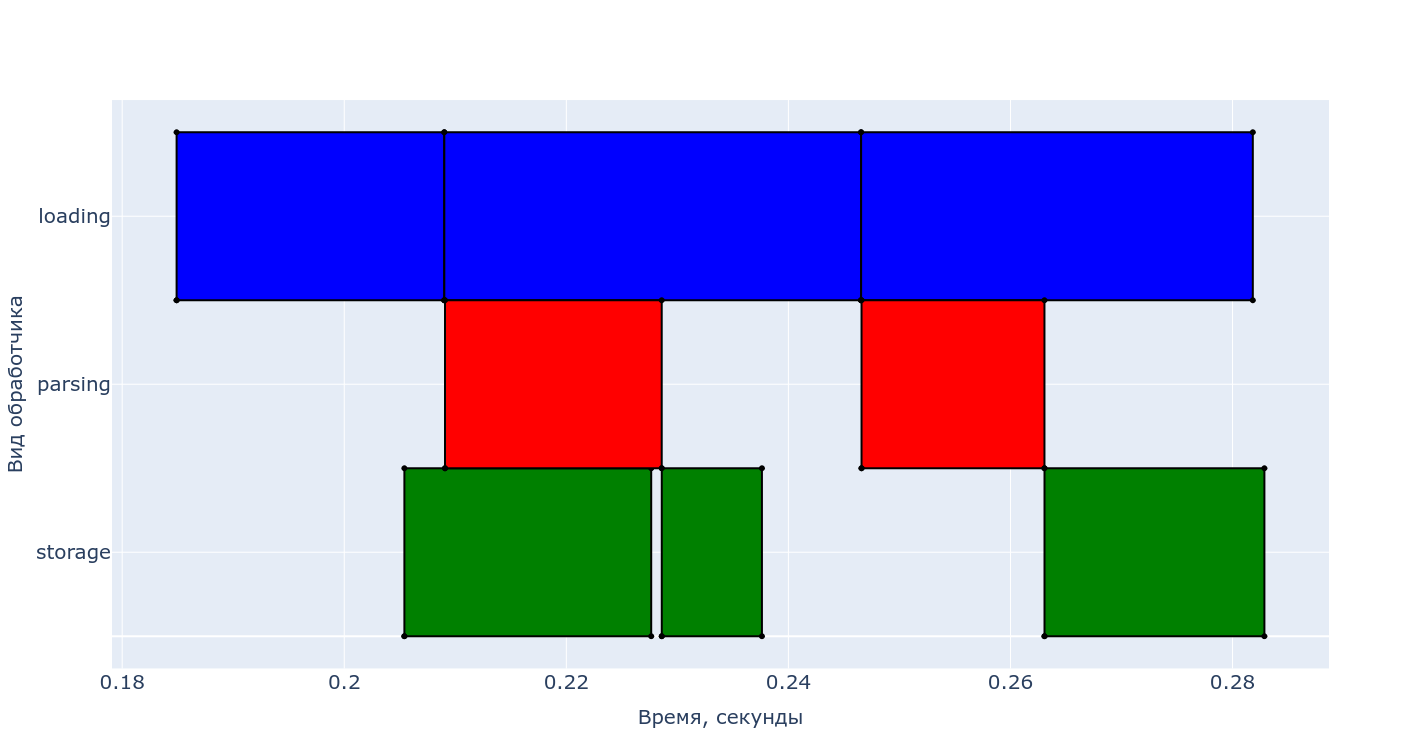
\includegraphics[width=0.9\textwidth]{timediag}
	\caption{Временная диаграмма простоя обработчиков}
	\label{timediag}
\end{figure}

Как видно на данном участке обработчик загрузки страниц беспрерывно их скачивают, а обработчики вычленения и сохранения рецепта простаивают в ожидании новых данных.

Также по данным всего лога программы была составлена таблица с временными характеристиками программы \ref{tbl:time}.


\begin{longtable}{|p{0.32\textwidth}|r|r|r|r|}
	\caption{Временные характеристики разработанной программы}\label{tbl:time}	\\
	\hline
	\multicolumn{1}{|c|}{Характеристика} & \multicolumn{1}{|c|}{Минимум, мс} & \multicolumn{1}{|c|}{Максимум, мс} & \multicolumn{1}{|c|}{Среднее, мс} & \multicolumn{1}{|c|}{Медиана, мс} \\
	\hline
	\endfirsthead
	\caption{Временные характеристики разработанной программы}
	\\
	\hline
	\multicolumn{1}{|c|}{Характеристика} & \multicolumn{1}{|c|}{Минимум, мс} & \multicolumn{1}{|c|}{Максимум, мс} & \multicolumn{1}{|c|}{Среднее, мс} & \multicolumn{1}{|c|}{Медиана, мс} \\
	\hline
	\endhead
	\hline
	\endfoot
	\endlastfoot
	Время загрузчики & 16.09 & 610.20 & 33.04 & 22.30 \\
	\hline
	Время парсинг & 12.31 & 41.62 & 15.70 & 15.05 \\
	\hline
	Время сохранения & 7.29 & 50.72 & 17.40 & 16.98 \\
	\hline
	Время ожидания парсера & 0.002 & 22.27 & 0.31 & 0.03 \\
	\hline
	Время ожидания сохранения & 0.02 & 30.99 & 0.70 & 0.06 \\
	\hline
	Время простоя парсера & 0.02 & 596.90 & 17.53 & 7.24 \\
	\hline
	Время простоя сохранения & 0.02 & 614.60 & 15.83 & 5.27 \\
	\hline
	Время обработки ссылки & 40.5 & 663.6 & 67.16 & 56.16 \\
	\hline
\end{longtable}

В результате исследования сделан вывод, что в случае выполнения конвейерных параллельных вычислений могут возникать простои отдельных её частей, то есть моменты времени, когда часть конвейера не выполняет вычисления, ожидая данных от предыдущих частей конвейера.
\clearpage

\ssr{ЗАКЛЮЧЕНИЕ}

Целью -- разработка ПО, выполняющего скачивание страниц и парсинг рецептов с сайта menunedeli.ru с помощью параллельных вычислений по конвейерному принципу -- была выполнена.

В ходе работы были решены следующие задачи:
\begin{itemize}
	\item рассмотрена структуры сайта;
	\item разработано ПО, выполняющее парсинг рецептов в конвейере;
	\item исследованы характеристики разработанного ПО на данных о интервалах времени стадий обработки рецепта.
\end{itemize}

В ходе исследования было выявлено, что использование конвейера для параллельных вычислений может привести к простою отдельных его частей из-за ожидания завершения обработки данных предыдущими частями конвейера.






